% !TEX root = ../C++Prime-Plus-Notes.tex
% !TEX encoding = UTF-8

\chapter{复合类型}

\addtocounter{section}{1}

\section{字符串}

\subsection{拼接字符串常量}

对于\codeline{char boss[8] = "Bozo"}这样的字符串赋值方法,后面的四个字符均会被赋成\\ \leftqm\mybackslash 0\rightqm\thinspace。另外,字符串常量(使用双引号)不能与字符常量(使用单引号)互换,字符常量如\thinspace\fira{'}S\fira{'}\thinspace 只是83的另一种写法,因此\codeline{char str = 'S'}表示将83赋给str。但\thinspace\fira{"}S\fira{"}\thinspace 不是字符常量,它表示的是两个字符(S和\thinspace\mybackslash n\thinspace)组成的字符串,并且\thinspace\fira{"}S\fira{"}\thinspace 表示的是这个字符串所在的内存地址,所以你如果写出\codeline{char str = "S"}这样的代码,编译器是要报错的,因为没有这种类型转换。\dpar

顺便说一说那个著名的“烫烫烫”和“屯屯屯”,在Debug 模式下,VS会把未初始化的栈内存全部填成0xCC。会把未初始化的堆内存全部填成0xCD。但是Release模式下不会有这种附加动作,原来那块内存里是什么就是什么(我在CentOS下用g++编译输出发现每次输出的字符串都不一样,并且大多都是乱码,到这里我也不知道为什么了,可能要牵扯到DRAM原理了)。未初始化的变量会被系统赋初值为0xCC,超过了ASCII码0-127这个范围,因此这个字符串被系统当成了宽字符组成的字符串,即两个字节数据组成一个字符,而0xCCCC表示的宽字符在GBK编码中正好是乱码中的那个烫字,0xCDCD在GBK编码中就是屯字。

当然,我们也可以追踪一下这种行为,可以在VS中打断点调试然后查看反汇编代码,栈中的填充很容易追踪,堆中的填充就不太好追踪了。Linux下你可以使用objdump命令来查看可执行文件的反汇编代码。

\addtocounter{subsection}{2}

\subsection{每次读取一行字符串输入}

对于普通的输入就比如\codeline{std::cin >> str},std::cin通过使用空白(空格,制表符和换行符)来确定字符串的结束位置,也就是说你想在一个字符串中输入空格用普通的std::cin是做不到的。istream中的类如\codeline{std::cin}提供了两个面向行的类成员函数:\codeline{getline()}和\\ \codeline{get()}。这两个函数都读取一行输入,直到达到换行符。然而,随后getline()将丢弃换行符,而get()将换行符保留在输入序列中。

getline()函数在istream中的原型为\codeline{\_\_istream\_type\& getline(char\_type*\ \ }\\ \codeline{\_\_s, streamsize \_\_n)}(书上说是在后面会讲还可以有第三个可选参数的getline()),它接受一个char型数组的指针和一个streamsize(顾名思义就是字符串长度,就是流长嘛),当它读到换行符,且此时长度没有超过字符串的长度或者streamsize,它就会把换行符换成\leftqm\mybackslash 0\rightqm,如果超过了streamsize或者字符串的长度,它就会在streamsize-1的地方截断,让后把第streamsize位置为\leftqm\mybackslash 0\rightqm,注意此时你的缓冲区是有那些被截断的字符的,如果你想要清空它们,可以使用\codeline{std::cin.clear()},后面讲\concept{EOF}的时候会再说这个函数。

get()函数与getline()函数工作方式相近,它们接受的参数相同,解释参数的方式也相同,并且读取方式也相同,但是get()并不读取并丢弃换行符,而是将其留在输入流内,也就意味着当你第一次调用std::cin.get(str, ArSize)后,第二次调用这个函数会得到一个空的字符串(其实如果你不去管那个换行符,以后再读取都是空字符串),这就是因为换行符依旧在输入流内,而下一个get()函数认为已经读到行尾了。但不带任何参数的std::cin.get()可以读取下一个字符(C++的函数重载让cin变得非常的智能),因此可以拿它来清理这个换行符。由于std::cin.get(str, ArSize)返回的是一个cin对象,你可以使用\codeline{std::cin.get(str,\ \ }\\ \codeline{ArSize).get()}的方法。同理,getline()函数也可以这样调用,\codeline{std::cin.getline(\ \ }\\ \codeline{str1, ArSize).getline(str2, ArSize)}表示把输入流中连续的两行分别读入str1和str2两个字符串。

可以看到,使用getline()函数更加方便,而使用get()函数能够让我们更加精细的去调控需要读取的字符。当get()函数读取到空行时,还会设置失效位(failbit),会将接下来的输出阻断,当然,你也可以用std::cin.clear()来重置输入流。\dpar

这里顺便讲一下关于回车换行的问题,在屏幕还不普及的时代,结果输出经常是依赖于所谓的电传打印机,打印头沿着打印杆从左向右移动并打印出一个个字符,当碰到一个回车符时(CR,0x0D,\mybackslash r),打印机就指示打印头重新回到最左边的位置上,这即是传统意义上的回车了。回车符后常跟着一个换行符(LF,0x0A,\mybackslash n),打印机收到换行符就会指示滚筒滚动,这样,打印头就对准了纸张上的新的一行,如果没有换行,新的打印输出就会重叠在上一行上,有时走纸不顺畅时也会造成这种后果。在Windows系统上,回车键会产生两个字符CRLF,一起表示换行,Unix/Linux之类的则单独用LF表示换行,而苹果的MacOS则单独用CR来表示换行,其实这里最符合传统的应该是微软,毕竟和电传打印机的回车换行是一致的,但是用一个字符表示换行符能够减少文件大小,这也是Unix/Linux和MacOS用一个字符来表示换行符的原因,至于为什么一个用回车,一个用换行,可能为了独树一帜吧。

\section{string类简介}

\addtocounter{subsection}{4}

\subsection{其他形式的字符串字面值}

同理,对于字符常量有用的前缀,对于字符串也可以用,L代表w\_char,u代表char\_16,U代表char\_32。C++11还支持UTF-8编码,你可以使用u8前缀来表示这种类型的字符串字面值,就比方说零宽无间断间隔符[Unicode zero-width no-break space character],它的编码是\leftqm\mybackslash xEF\mybackslash xBB\mybackslash xBF\rightqm,用u8前缀就可以写成u8\leftqm\mybackslash uFEFF\rightqm。\dpar

C++11还新增了原始(Raw)字符串,就是禁止转义啦,原始字符串需要以R开头,并且用\thinspace\fira{"(}\thinspace 和\thinspace\fira{)"}\thinspace 作为定界符,就比如\codeline{std::cout << R"(\mybackslash n)" << std::endl}会直接输出\thinspace\mybackslash n,这里这样定义定界符是为了能让你在字符串里直接输入\thinspace\fira{"}\thinspace,并且在输入原始字符串时,按回车键会在里面加入回车字符。当然,如果你想在原始字符串中包含\thinspace\fira{"(}\thinspace 或\thinspace\fira{)"}\thinspace,原始字符串允许你在\thinspace\fira{"}\thinspace 和\thinspace\fira{(}\thinspace 之间包含其他字符,只要你也以这些字符结尾即可。同时,这些前缀可以混合搭配,并且不区分顺序。

\section{结构简介}

\subsection{在程序中使用结构}

说一下考试很喜欢考的结构体占用的内存问题,这个就牵扯到内存对齐的事情了,一般编译器都会自动帮你把内存对齐的(如果你想手动指定对齐或者禁止对齐请使用\codeline{\#pragma\ \ }\\ \codeline{pack(n)},n为对齐的宽度),下面这个例子运行在CentOS 64位机上。

\begin{cpp}
#include <iostream>

int main(int argc, char|*| argv[]) {
    struct {
        int a;
        double b;
        short c;
    } A;
    struct {
        int a;
        short b;
        double c;
    } B;
    std::cout << sizeof(A) << std::endl; // 24
    std::cout << sizeof(B) << std::endl; // 16
    return 0;
}
\end{cpp}

在结构体中,从结构体的首地址开始,假设地址从0开始。对结构体A来说,a占4个字节,占从0\~{}3的字节,b是double类型占8个字节,占从8\~{}15的字节,c占两个字节,从16\~{}17的字节。对结构体B来说,a占4个字节,从0\~{}3,b占两个字节从4\~{}6;c占8个字节从8\~{}15。这就是内存对齐,对齐规则是按照成员的声明顺序,依次安排内存,其偏移量为成员大小的整数倍,0看做任何成员的整数倍,最后结构体的大小为最大成员的整数倍(所以这里的A的大小是24,而不是18)。在C++中规定了空结构体和空类的内存所占大小为1字节,因为C++中规定,任何不同的对象不能拥有相同的内存地址。

系统进行内存对齐,可以提高CPU处理速率,而这项任务就交给编译器进行相应的地址分配和优化,编译器会根据提供参数或者目标环境进行相应的内存对齐,当然内存对齐也有硬件方面的原因,有些硬件规定了读取地址,如果指令地址和其规定地址不一致,则该硬件可能会发生崩溃等未知情况。

\addtocounter{section}{2}

\section{指针和自由存储空间}

\subsection{声明和初始化指针}

前面已经说过,无论是在32位还是64位机上,int型都是4个字节,而int型指针变量(其实无论什么型的指针都是一样,无非就是存了一个内存地址变量)在32位机上是4个字节,在64位机上是8个字节(不用担心内存地址存不下的情况,因为你根本弄不到那么大的内存,linux的64位机的虚拟地址只有48位,为了节约空间),所以在64位机上指针的内建类型应该是unsigned long。这里顺便讲一下一个C++程序在内存中的空间分配,具体见\fref{figure:RAM}\cite{LinuxProgram}。

\begin{figure}[!hbt]
\centering
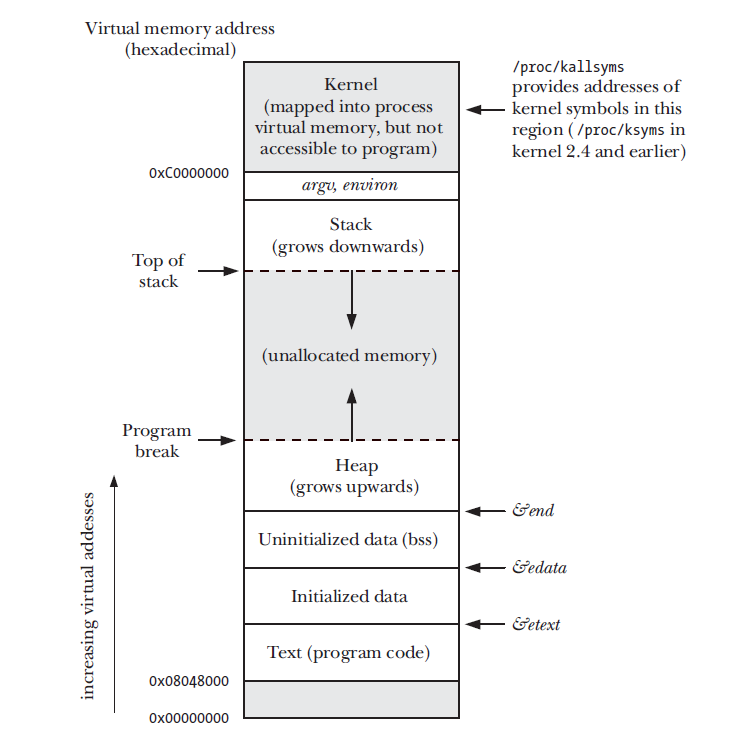
\includegraphics[scale=0.9]{./Figures/RAM}
\caption{Typical memory layout of a process on Linux/x86-32}
\label{figure:RAM}
\end{figure}

栈是向低地址扩展的数据结构,是一块连续的内存区域,这句话的意思是栈顶的地址和栈的最大容量是系统预先规定好的,当申请的空间超过栈的剩余空间时,将提示溢出。因此,用户能从栈获得的空间较小。堆是向高地址扩展的数据结构,是不连续的内存区域。因为系统是用链表来存储空闲内存地址的,且链表的遍历方向是由低地址向高地址。由此可见,堆获得的空间较灵活,也较大。栈中元素都是一一对应的,不会存在一个内存块从栈中间弹出的情况,这里再说下去要讲到C++里内存分配了,这些还是放到后面讲到malloc()的时候再说吧\footnote{具体可以参见\thinspace\href{https://www.cnblogs.com/zhaoosheLBJ/p/9281253.html}{Linux C 内存分配}这篇文章}。

\subsection{指针的危险}

在你没有将一个指针指向某一块你分配好的内存之前,不要对这个指针解除引用并赋值(也就是说,不要用一个右值来初始化指针),下面这个程序会说明这件事情:

\begin{cpp}
#include <iostream>

int main(int argc, char|*| argv[]) {
    long|*| fellow;
    |*|fellow = 8888;
    std::cout << |*|fellow << std::endl;
    return 0;
}
\end{cpp}

这个程序能够正常过编译,但是运行时会报如下\codeline{[1] 14741 segmentation fault\ \ }\\ \codeline{./init\_ptr}的错误,其中14741代表进程号,而segmentation fault就是段错误,所谓的段错误就是指访问的内存超过了系统所给这个程序的内存空间,通常这个值是由gdtr(全局描述符寄存器)来保存的,它是一个48位的寄存器,其中的32位是保存由它指向的gdt表(全局描述符表),后13位保存相应于gdt的下标,最后3位包括了程序是否在内存中以及程序的在CPU中的运行级别,指向的gdt是由以64位为一个单位的表,在这张表中就保存着程序运行的代码段以及数据段的起始地址以及相应的断限和页面交换还有程序运行级别和内存粒度等信息,一旦一个程序发生了越界访问,CPU就会产生相应的异常保护,于是segmentation fault就出现了。

有许多情况会导致SIGSEGV,上面一种就是引用了空指针导致访问了不存在的内存而报错\footnote{具体可以参见\thinspace\href{https://www.cnblogs.com/qiumingcheng/p/11254648.html}{Segmentation Fault错误原因总结}这篇文章}。

\subsection{指针和数字}

如果你想手动指定指针指向的内存地址,C++在类型一致方面要求更加严格,因此你需要显式地将数字转换成地址类型,你可以将\codeline{(int*) 0xB8000000}赋给一个int型指针。

\subsection{使用new来分配内存}

new分配的内存通常与常规变量声明分配的内存块不同,新建的变量和指针的值都储存在栈(stack)中,而new分配的内存是在堆(heap)或自由储存区(free store)中。如果你new请求内存失败,C++将返回0,即生成了一个空指针,书上说后面会讨论这一异常。

\subsection{使用delete释放内存}

使用new分配的内存在用完后需要用delete运算符归还这一块内存,你可以直接delete一个指针,这会释放这个指针指向的内存,而不会删除这个指针。如果你忘记delete一块new出来的内存,就会发生内存泄漏(当你编写一些复杂的程序时,内存泄漏可能会难以发现,好吧,VS有性能探查器,可以帮你检测内存泄漏,毕竟宇宙第一IDE)。但是尽管你delete掉这一块内存,你会发现它依旧是可以访问的,释放的内存系统可能不会直接使用,但后面会发生什么就没人知道了,如果你不想让这种事情发生,当你delete后请将指针置为NULL。

\subsection{使用new来创建动态数组}

在编译时给数组分配内存称为静态联编(static binding),这意味着数组实在编译的时候加入到程序中的。使用new时,你可以在程序运行时确定数组的长长度,这称为\concept{动态联编(dynamic binding)},生成的数组叫做动态数组。

为动态数组分配内存的通用格式为:\codeline{type\_name * pointer\_name = new type\_}\\ \codeline{name [num\_elements]},同样释放内存的格式也改为\codeline{delete [] pointer\_name},还有就是你没法用sizeof来确定动态分配的数组的长度,它只会返回其中一个元素的长度。

\section{指针,数组和指针算术}

\addtocounter{subsection}{1}

\subsection{指针小结}

对指针来说,它的类型决定了每次偏移的地址量,即当你将pointername\thinspace$\pm$\thinspace1时指针移动的位数。因此对于一个数组,\codeline{arrayname[4]}和\codeline{*(arrayname + 4)}是一个意思。

对数组取地址时,数组名会被解释称其第一个元素的地址,即\codeline{\&array\_name[0]},而直接对数组名取地址(\codeline{\&array\_name})会返回同样的地址,但这次返回的是整个数组的地址,下面这个程序会解释这个现象:

\begin{cpp}
#include <iostream>

int main(int argc, char|*| argv[]) {
    short pt[10];
    short |*|pd = new short [10];
    std::cout << !!&!!pt << std::endl; // 0x7ffec62c9010
    std::cout << !!&!!pt + 1 << std::endl; // 0x7ffec62c9024
    std::cout << pt << std::endl; // 0x7ffec62c9010
    std::cout << pt + 1 << std::endl; // 0x7ffec62c9012
    std::cout << !!&!!pd << std::endl; // 0x7ffec62c9008
    std::cout << !!&!!pd + 1 << std::endl; // 0x7ffec62c9010
    std::cout << pd << std::endl; // 0xd8a010
    std::cout << pd + 1 << std::endl; // 0xd8a012
    delete !![]!! pd;
    return 0;
}
\end{cpp}

上面程序中pt + 1就是很普通的指针加法,而\&pt + 1则直接跳到了整个数组的尾部,这也说明了对数组名取地址最然返回的也是第一个元素的地址,但其实它的长度是整个数组。另一个差别就是,要得到第一个元素的值,只需要对pt解除一次引用,但需要对\&pt解除两次引用,即\codeline{**\&pt == *pt == pt[0]}。

\addtocounter{subsection}{1}

\subsection{使用new创建动态结构}

对于新创建的动态结构或者指向结构的指针,你可以使用\codeline{pointer\_name->member\_}\\ \codeline{name},\codeline{struct\_name.member\_name}或者\codeline{*(pointer\_name).member\_name}的方式来访问里面的成员,其中\thinspace\fira{->}\thinspace 叫做间接成员运算符,而.为成员运算符。

\addtocounter{section}{1}

\section{数组的替代品}

\subsection{模板类vector}

模板类vector类似于string类,也是一种动态数组,并且通过new和delete来管理内存,你可以使用\codeline{std::vector<type\_name> vector\_name(elenemnt\_number)},其中element\_number可以是一个在编译期间不能确定的变量,好了,书上说的就只有怎么多了。\dpar

既然讲到了vector,顺便说一下C++的\href{https://zh.cppreference.com/w/cpp/container}{容器}(不是Docker的那个容器),书上应该会在后面开一章来讲这个,这里就先随便讲一下吧。在C++中容器的定义为:在数据存储上,有一种对象类型,它可以持有其它对象或指向其它对像的指针,这种对象类型就叫做容器。每一种容器都有其优点和缺点,所以为了应付程序中的不同需求,STL实现了七种基本容器类型。

\subsection{模板类array(C++11)}

你可以通过\codeline{std::array<type\_name elenemnt\_number> array\_name}来新建\\ 一个array对象。

\subsection{比较数组,vector对象和array对象}

无论是数组,vector对象和array对象,都可以使用标准数组表示法来访问各个元素(但其实这些容器都有自己实现的访问方法),对于数组的越界访问,C++是不会禁止的,也就是说你可能会通过数组的下标来访问一些数组外的内存地址,这种用容器都是可以避免的。
